\documentclass[10pt]{article}
\usepackage{icmlko}

\icmlmeta{IP 파운데이션 월드모델}{9}{건너간 것과 건너가지 못한 것}{아이돌에서도 축은 상수를 이긴다 --- 그러나 넷 중 둘만 같은 부호로 옮겨갔다}

\begin{document}

\twocolumn[
\icmlheader

\begin{abstract}
이 노트는 이 연구의 전제를 처음으로 직접 시험한다. 세 단계를 거쳤다. 첫째,
\textbf{노트 8의 설명을 철회한다} --- 축 복원 실패의 원인을 ``축퇴''로 추정했으나
직교화로 승률이 전혀 회복되지 않았고(변화 0.00) 복원 축은 사람 태그보다 오히려
\emph{덜} 상관돼 있었다. 축별 상관을 재보니 넷이 r=0.43--0.55로 실질 복원된다.
원인은 축퇴도 정보 부족도 아니라 \textbf{회귀 희석}이었다. 둘째, 그렇다면 얼마나
정확해야 쓸모가 있는지 답할 수 있다. 사람 태그를 통제된 잡음으로 열화시켜 재보니
\textbf{승률 90\%에는 r$\geq$0.79, 50\%에는 r$\geq$0.52가 필요하다}. 현재 문서
복원 수준 0.45는 문턱 아래다. 셋째, 노트 8이 지정한 수집 과제를 실행해 아이돌
데뷔 앨범의 버전 수와 정가를 81건 중 69건 확보하고, 태깅률 0\%였던 두 축을 채운 뒤
전이를 검정했다. 결과가 갈린다. \textbf{아이돌 도메인에서도 네 축은 상수를 이긴다}
(차이 $-$0.0574, 승률 97\%) --- 축이 팝업 국소적이지 않다는 첫 증거다. 그런데
\textbf{전이는 실패한다}. 부호가 일치하는 축이 넷 중 둘뿐이고 계수 상관은
$-$0.309다. 살아남은 둘은 미디어 투입과 굿즈 규모이며, 입장 허들은 부호가 뒤집혔다 ---
앨범 가격은 허들이 아니라 규모 신호였다.
\end{abstract}
]

\section{먼저 노트 8을 고친다}

노트 8은 문서에서 복원한 축으로 결과를 예측하면 승률 100\%가 5\%로 무너진다고
보고하고, 원인을 이렇게 추정했다.

\begin{quote}\fontsize{9.2}{11}\selectfont
각 축을 같은 문서 피처로 예측하면 복원 오차가 서로 독립이 아니다. \dots\ 그러면
복원된 다섯 축은 실질적으로 하나의 ``규모'' 축으로 축퇴하고, 다섯 축이 서로 다른
것을 재기 때문에 생기던 이득이 사라진다.
\end{quote}

같은 노트의 반증 조건도 함께 적어 두었다 --- 직교화로 회복되면 표현 문제, 안 되면
정보 문제. 돌렸다.

\begin{table}[t]
\centering\tsize
\caption{축퇴 가설의 직접 검정. IP 무작위 5폴드 20회 반복.}
\begin{tabular}{lrrr}
\toprule
& 평균 $|r|$ & 최대 $|r|$ & 제1주성분 설명 \\
\midrule
사람 태그 & 0.236 & 0.540 & 0.372 \\
문서 복원 & 0.177 & 0.465 & 0.322 \\
\midrule
\multicolumn{4}{l}{\vspace{-0.6em}} \\
& 차이 중앙 & 표준편차 & 이긴 비율 \\
\midrule
참 축            & $-$0.0313 & 0.011 & 100\% \\
복원 축          & $+$0.0254 & 0.028 & 5\% \\
복원 축 직교화   & $+$0.0243 & 0.028 & 5\% \\
\bottomrule
\end{tabular}
\end{table}

두 방향 모두 가설과 어긋난다. 축퇴가 사실이면 복원 축이 사람 태그보다 \emph{더}
상관돼 있어야 하는데 덜 상관돼 있다(0.177 대 0.236). 그리고 직교화로 승률이
전혀 움직이지 않는다(5\% $\to$ 5\%).

\claimx{노트 8의 ``축퇴'' 설명을 철회한다. 복원 축은 사람 태그보다 덜 상관돼 있고
직교화로 아무것도 회복되지 않는다.}{다른 직교화 방식(주성분, 백색화)에서 회복되면
철회가 성급했던 것이다.}

\subsection{그러면 정보가 없는가 --- 그것도 아니었다}

다음 후보는 ``문서에 정보가 없다''였다. 축별 복원 상관을 재봤다.

\begin{table}[t]
\centering\tsize
\caption{문서 피처로 각 축을 예측했을 때 참값과의 상관(20회 반복 중앙값).}
\begin{tabular}{lrr}
\toprule
축 & ridge & 트리 \\
\midrule
입장 허들   & 0.311 & \textbf{0.548} \\
굿즈 규모   & 0.383 & \textbf{0.470} \\
매장 노출도 & \textbf{0.438} & 0.378 \\
타깃 폭     & 0.235 & \textbf{0.429} \\
\midrule
미디어 투입 & 0.143 & 0.193 \\
\bottomrule
\end{tabular}
\end{table}

넷이 0.43--0.55로 복원된다. 잡음이 아니다. 그런데도 쓸모가 없다.

남는 설명은 \textbf{회귀 희석}이다. 측정 오차가 있는 예측변수는 그 효과를 신뢰도만큼
감쇠시킨다. 참 축의 효과가 애초에 크지 않으므로(차이 $-$0.0313), 신뢰도 0.45로
감쇠되면 남는 것이 없다.

\section{그래서 얼마나 정확해야 하는가}

이 진단은 답할 수 있는 질문으로 바뀐다. 사람 태그를 통제된 잡음으로 열화시켜
목표 상관 $r$을 맞춘 뒤, $r$이 얼마일 때 상수를 이기기 시작하는지 재면 된다.
표준화한 참값 $z$에 대해 $z' = r z + \sqrt{1-r^2}\,e$로 만들면
$\mathrm{corr}(z, z') = r$이 된다.

\begin{table}[t]
\centering\tsize
\caption{축 측정 신뢰도에 따른 성능. IP 무작위 5폴드 40회 반복, ridge.}
\begin{tabular}{rrrr}
\toprule
신뢰도 $r$ & 차이 중앙 & 이긴 비율 \\
\midrule
1.00 & $-$0.0371 & 100\% \\
0.95 & $-$0.0339 & 100\% \\
0.90 & $-$0.0269 & 97\% \\
0.80 & $-$0.0180 & 93\% \\
0.70 & $-$0.0101 & 68\% \\
0.60 & $-$0.0085 & 75\% \\
0.50 & $+$0.0031 & 45\% \\
0.45 & $+$0.0144 & 45\% \\
0.30 & $+$0.0178 & 23\% \\
\bottomrule
\end{tabular}
\end{table}

\begin{figure}[t]
\centering
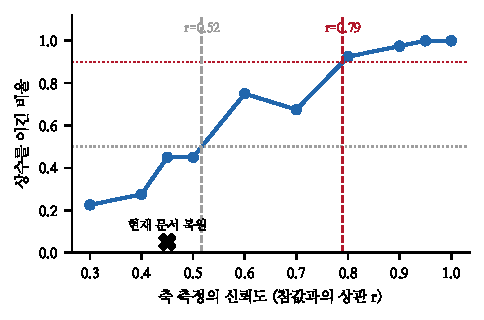
\includegraphics[width=\columnwidth]{figs/reliability.pdf}
\caption{신뢰도 문턱. 승률 90\%를 지키려면 r$\geq$0.79, 절반이라도 이기려면
r$\geq$0.52가 필요하다. X 표시가 현재 문서 복원 수준이다.}
\end{figure}

\claimx{축 측정의 신뢰도가 0.79 아래로 내려가면 이 표본에서 축은 실용적 가치를
잃는다. 이것은 태깅 품질에 대한 공학 규격이다 --- 평정자 간 일치도가 이 문턱
아래면 태깅 설계를 다시 해야 한다.}{표본이 커지면 같은 신뢰도에서도 효과가
살아난다. n=150에서 문턱이 0.6 아래로 내려가면 이 수치는 표본 크기에 딸린
값이지 축의 성질이 아니다.}

이 숫자는 실무 지침이 된다. 사람 태깅의 평정자 간 일치도를 아직 재지 않았는데,
그것이 0.8을 넘지 못하면 지금 쓰고 있는 태그 자체가 문턱 아래일 수 있다.
다음 측정 과제다.

\section{수집을 실행했다}

노트 8은 아이돌 도메인에서 입장 허들과 굿즈 규모의 태깅률이 0\%라고 보고하고
수집 과제로 지정했다. 실행했다.

음반 유통 상품 페이지에 버전 수와 정가가 그대로 있다. 그룹명과 앨범명이 \emph{둘 다}
상품 제목에 있어야 채택하는 규약으로 81건 중 69건(85\%)을 확보했다. 이 프로젝트의
크롤링 사고는 전부 ``비슷해 보이는 것을 같은 것으로 본'' 데서 났으므로 --- 4개 그룹
합동 기사 수치를 한 그룹에 귀속시킨 사건, 그룹 전체 유동인구를 한 팝업에 넣은 사건 ---
채택한 상품 제목과 상품 번호를 전부 기록했다.

버전 수 세기에서 한 번 과대 계상이 났다. 한 걸그룹의 데뷔 앨범이 12종으로 잡혔는데,
제목의 ``버전별 CD알판 12종 중 랜덤삽입''을 센 것이었다. 12종은 알판 그림이지 앨범
버전이 아니다. 실제 버전은 COLOR와 ROSE 두 종이다. 규칙을 고쳐 --- 버전 표기가
있으면 그것을 세고 없을 때만 N종 표기로 넘어가도록 --- 바로잡았다.

\begin{table}[t]
\centering\tsize
\caption{아이돌 한터 확정 81건의 축 태깅률 변화.}
\begin{tabular}{lrr}
\toprule
축 & 수집 전 & 수집 후 \\
\midrule
미디어 투입 & 96\% & 96\% \\
타깃 폭     & 91\% & 91\% \\
입장 허들   & \textbf{0\%} & \textbf{85\%} \\
굿즈 규모   & \textbf{0\%} & \textbf{85\%} \\
매장 노출도 & 32\% & 32\% \\
\bottomrule
\end{tabular}
\end{table}

\section{전이 검정}

두 도메인의 라벨은 물리량이 다르다. 그래서 도메인 안에서 y를 표준화하고 축도 각각
표준화한다. 검정하는 것은 절대값이 옮겨지는가가 아니라 \emph{축과 결과의 관계가
옮겨지는가}이며, 후자가 파운데이션 가설이 실제로 주장하는 바다. 매장 노출도는
아이돌 태깅률이 32\%뿐이라 뺐다.

\begin{figure}[t]
\centering
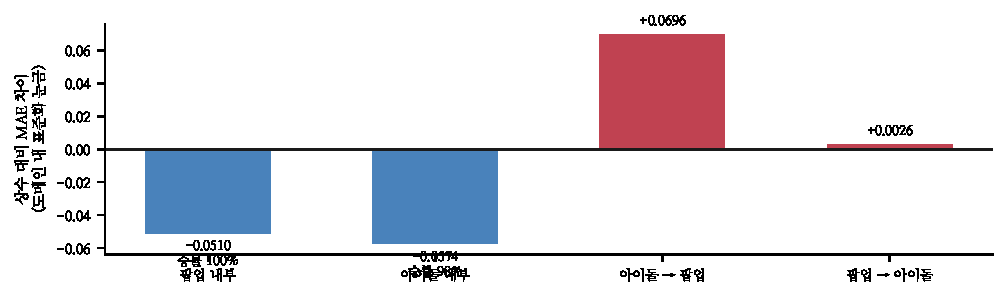
\includegraphics[width=\textwidth]{figs/bars.pdf}
\caption{도메인 안에서는 둘 다 이기고, 건너가면 둘 다 진다.}
\end{figure}

\begin{table}[t]
\centering\tsize
\caption{도메인 내부와 교차. 팝업 75건, 아이돌 63건(네 축 완전 케이스).}
\begin{tabular}{lrr}
\toprule
& 차이 & 이긴 비율 \\
\midrule
팝업 내부   & $-$0.0510 & 100\% \\
아이돌 내부 & $-$0.0574 & 97\% \\
\midrule
아이돌 $\to$ 팝업 & $+$0.0696 & --- \\
팝업 $\to$ 아이돌 & $+$0.0026 & --- \\
\bottomrule
\end{tabular}
\end{table}

\paragraph{좋은 소식} 아이돌 도메인에서도 네 축은 상수를 이긴다(차이 $-$0.0574,
40회 중 39회). 팝업에서 만든 축 어휘가 다른 도메인에서 처음으로 검증됐다. 축이
팝업 국소적인 발견이 아니라는 첫 증거다.

\paragraph{나쁜 소식} 교차는 둘 다 진다. 아이돌에서 배운 계수로 팝업을 예측하면
대상 도메인 상수보다 0.0696 나쁘고, 반대 방향은 0.0026 나쁘다(거의 비김).

\section{왜 안 건너갔는가}

계수를 보면 진단이 나온다.

\begin{figure}[t]
\centering
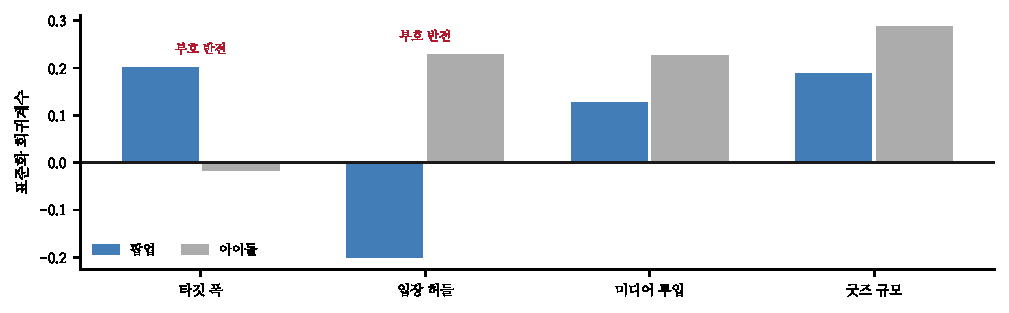
\includegraphics[width=\textwidth]{figs/coef.pdf}
\caption{표준화 회귀계수. 미디어 투입과 굿즈 규모는 같은 부호로 건너갔고,
입장 허들은 뒤집혔으며, 타깃 폭은 아이돌에서 사실상 0이다.}
\end{figure}

\begin{table}[t]
\centering\tsize
\caption{도메인별 표준화 회귀계수. 부호 일치 2/4, 계수 상관 $-$0.309.}
\begin{tabular}{lrrl}
\toprule
축 & 팝업 & 아이돌 & \\
\midrule
미디어 투입 & $+$0.127 & $+$0.226 & 일치 \\
굿즈 규모   & $+$0.189 & $+$0.287 & 일치 \\
\midrule
타깃 폭     & $+$0.202 & $-$0.016 & 아이돌에서 무효 \\
입장 허들   & $-$0.201 & $+$0.229 & \textbf{부호 반전} \\
\bottomrule
\end{tabular}
\end{table}

\paragraph{입장 허들의 부호 반전이 결정적 단서다}
팝업에서는 입장 허들이 높을수록 방문자가 준다($-$0.201). 아이돌에서는 앨범 가격이
높을수록 초동이 는다($+$0.229). 같은 축이라면 있을 수 없는 일이다.

확인해 보니 원인은 내 매핑이었다. 아이돌 데이터에서 앨범 가격은 진입 비용이 아니라
\emph{규모 신호}다.

\begin{itemize}[leftmargin=1.1em,itemsep=0.15em]
\item 버전 수가 늘수록 평균 정가가 오른다: 1종 13,495원 $\to$ 2종 18,157원
      $\to$ 3종 이상 19,693원.
\item 가격과 버전 수의 상관 $+$0.198, 가격과 초동의 상관 $+$0.262,
      버전 수와 초동의 상관 $+$0.345.
\end{itemize}

비싼 앨범은 두꺼운 포토북과 많은 특전을 뜻한다. 즉 앨범 가격은 ``입장 허들''이
아니라 ``굿즈 규모''의 다른 얼굴이었다. 나는 두 축에 같은 신호를 넣고 서로 다른
것을 재기를 기대한 셈이다.

\claimx{전이 실패의 원인은 축이 도메인 특수해서가 아니라 아이돌 쪽 축 매핑이
틀렸기 때문이다. 앨범 가격은 입장 허들이 아니라 굿즈 규모다.}{앨범 가격을 굿즈
규모로 옮기고 입장 허들의 다른 대응물을 넣었을 때도 부호가 어긋나면, 그때는
매핑이 아니라 축 자체가 도메인 특수한 것이다.}

\paragraph{타깃 폭도 다시 짜야 한다}
아이돌 쪽 계수가 $-$0.016으로 사실상 0이다. 인원 수·성별·서바이벌 출신으로 만든
대리변수가 팝업의 ``대상이 얼마나 넓은가''와 같은 것을 재지 않는다.

\section{그래서 무엇이 남았나}

\begin{itemize}[leftmargin=1.1em,itemsep=0.15em]
\item \textbf{도메인 불변 후보 2개} --- 미디어 투입, 굿즈 규모. 두 도메인에서
      같은 부호이고 크기도 비슷하다. 파운데이션 모델의 공유 슬롯은 여기서 시작한다.
\item \textbf{재설계 대상 2개} --- 입장 허들(아이돌 대응물을 팬덤 진입 비용 쪽에서
      다시 찾는다), 타깃 폭(대리변수 재설계).
\item \textbf{측정 규격 1개} --- 축 신뢰도 0.79. 사람 태깅의 평정자 간 일치도를
      재서 이 문턱을 넘는지 확인해야 한다.
\end{itemize}

\section{한계}

\begin{itemize}[leftmargin=1.1em,itemsep=0.15em]
\item 아이돌 축은 규칙 기반 유도이며 사람 태깅이 아니다. 팝업 쪽 태그와 같은 종류의
      물건이라는 보장이 없고, 신뢰도도 재지 않았다. 전이 실패의 일부가 여기서
      올 수 있다.
\item 교차 검정은 단일 적합이라 신뢰구간이 없다. 반복 분할로 다시 재야 한다.
\item 아이돌 완전 케이스가 63건이다. 계수 추정 자체의 분산이 크다.
\item 신뢰도 문턱 0.79는 이 표본(n=75)에 딸린 값이다. 표본이 커지면 내려간다.
\end{itemize}

\section{다음}

\begin{enumerate}[leftmargin=1.3em,itemsep=0.15em]
\item 앨범 가격을 굿즈 규모로 재배치하고 전이 재검정 --- 부호 반전이 해소되는가.
\item 입장 허들의 아이돌 대응물 재설계 --- 팬클럽 가입 비용, 예약 경쟁 구조.
\item 교차 검정에 반복 분할과 신뢰구간 부여.
\item 사람 태깅의 평정자 간 일치도 측정 --- 0.79 문턱을 넘는지.
\end{enumerate}

\vspace{0.6em}
\hrule height 0.3pt
\vspace{0.5em}
{\footnotesize
\textbf{참고문헌}\\[0.3em]
Ben-David, S. et al. (2010). A theory of learning from different domains.
\emph{Machine Learning}, 79(1--2), 151--175.\\[0.15em]
Carroll, R. J. et al. (2006). \emph{Measurement Error in Nonlinear Models},
2nd ed. Chapman \& Hall.\\[0.15em]
Spearman, C. (1904). The proof and measurement of association between two things.
\emph{American Journal of Psychology}, 15(1), 72--101.\\[0.15em]
Standley, T. et al. (2020). Which tasks should be learned together in multi-task
learning? \emph{ICML 2020}, 9120--9132.
}

\end{document}
